\PassOptionsToPackage{english}{babel}
\documentclass{report}
\usepackage[utf8]{inputenc}

%\usepackage[english]{babel}
%\usepackage[latin1]{inputenc}
%\usepackage{geometry}
%\usepackage{listings}
\usepackage{caption}
\usepackage{amsmath}
\usepackage{graphics}
\usepackage[T1]{fontenc}
\usepackage{enumitem} %bold enumeration
\usepackage[utf8]{inputenc}
\usepackage[english]{babel}
%\usepackage{pmgraph}
\usepackage{mathrsfs}
\usepackage{floatflt}
\usepackage{multicol}
\usepackage{color,colortbl}
% \usepackage[pdftex]{graphicx}
\usepackage[normalem]{ulem}
\usepackage[colorlinks,urlcolor=blue, linkcolor=blue]{hyperref}
\usepackage{epstopdf}
\usepackage{wrapfig}
\usepackage{multirow}
%% Sets page size and margins
\usepackage[a4paper,top=3cm,bottom=2cm,left=3cm,right=3cm,marginparwidth=1.75cm]{geometry}
%% Useful packages
\usepackage[colorinlistoftodos]{todonotes}
\usepackage{xymtex}
\usepackage{fancyhdr}
\usepackage{epstopdf}
\usepackage{indentfirst} \geometry{verbose,a4paper,tmargin=3cm,bmargin=3cm,lmargin=1.0cm,rmargin=2.0cm}
\setlength{\parindent}{0pt}
 \graphicspath{C:/Users/Anton/Desktop/ETH_books/CV/CV-Lab-Model-Fitting/CV-Lab-Model-Fitting/src/epipolar_geometry/res}
\begin{document}
\large
\if 0
Report of Anton Maksimov (antonma, 16-952-137), Task 5 "Image segmentation" on ETHZ course "Computer Vision".\\
\rule{\linewidth}{1pt}
%%%%%%%%%%%%%%%%%%%%%%%%%%%%%%%%%%%%%%%%%%%%%%%%%%%%%%%%%   1
	\textbf{8.1}
	\begin{figure}[h!]
		\begin{center}
			\begin{minipage}[h]{0.49\linewidth}
				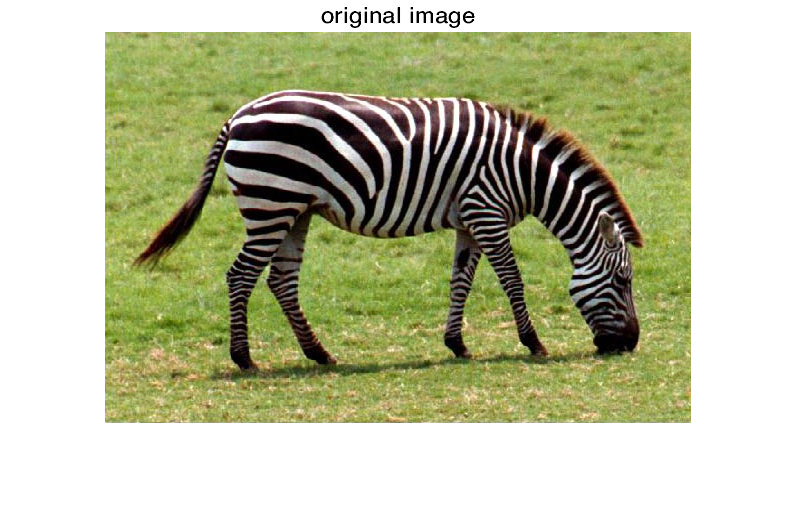
\includegraphics[width=1\linewidth]{C:/Users/Anton/Desktop/ETH_books/CV/cv_lab05_exercise/last_res/orig}
				\caption{Original image.}
			\end{minipage}
			\hfill
			\begin{minipage}[h]{0.49\linewidth}
				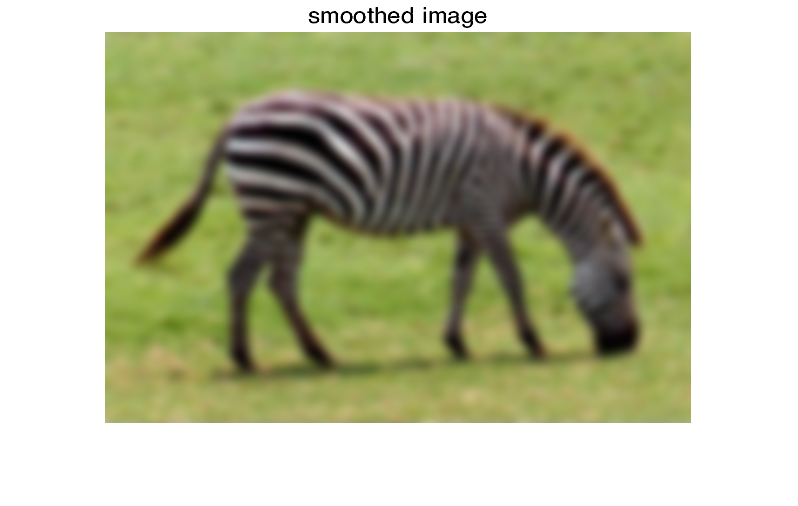
\includegraphics[width=1\linewidth]{C:/Users/Anton/Desktop/ETH_books/CV/cv_lab05_exercise/last_res/smoothed}
				\caption{Blurred with Gaussion with $\sigma = 5$ image .}
			\end{minipage}
		\hfill
			\begin{minipage}[h]{0.49\linewidth}
				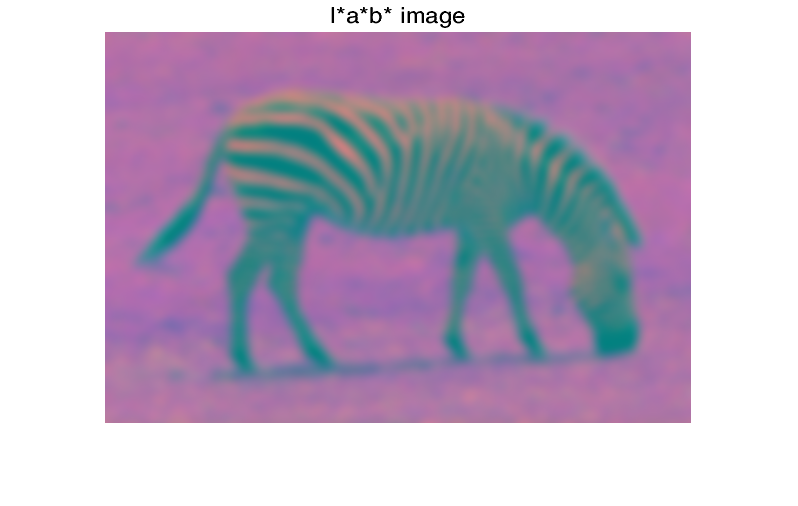
\includegraphics[width=1\linewidth]{C:/Users/Anton/Desktop/ETH_books/CV/cv_lab05_exercise/last_res/lab}
				\caption{Converted to L*a*b blurred image. This color scheme shows better how human perceives the image (distances in this color space are better correlated with how we see difference of colors), so it's more beneficial than RGB scheme for image segmentation as human do it. (ref. exercise session, Wikipedia)}
			\end{minipage}
		\end{center}
	\end{figure}\\

\textbf{8.2}
We implement mean-shift algorithm using different thresholds and radii $r$ for moving of the feasible peak location. After each step we create new peak if there are no peaks nearby (less that $r/2$). Otherwise, we merge it with the first found and change the position of the peak using votes (weights to find new center of mass of all pixels which were assigned to this peak).

Algorithm works good (though rather slow, so we used resized smaller images), we can distinguish zebra and cow with black and white spots.

In order to achieve results which are possible to compare using different rescaling factors, we use corresp. rescaled $\sigma$ of Gaussian filter applied before segmentation.

\begin{figure}[h!]
	\begin{center}
		\begin{minipage}[h]{0.49\linewidth}
			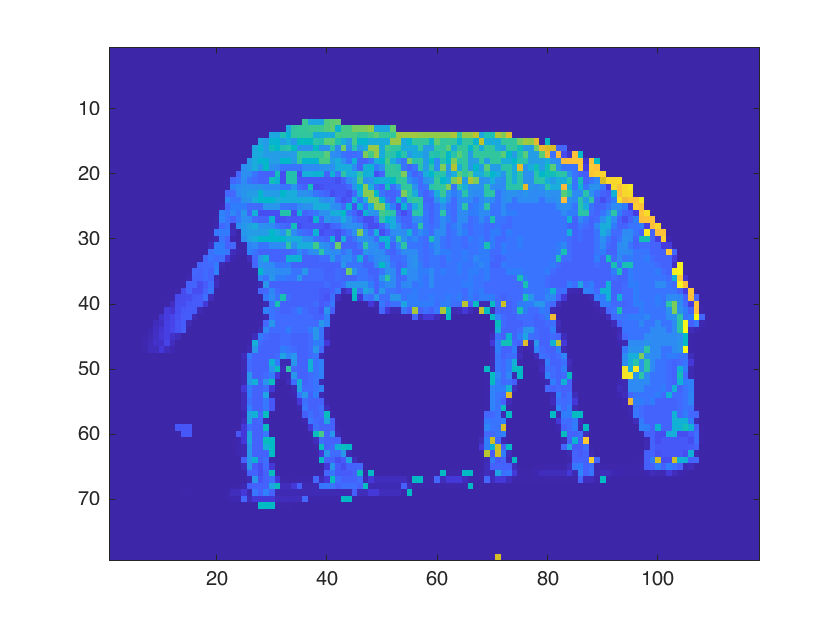
\includegraphics[width=1\linewidth]{C:/Users/Anton/Desktop/ETH_books/CV/cv_lab05_exercise/last_res/z_1}
			
		\end{minipage}
		\hfill
		\begin{minipage}[h]{0.49\linewidth}
			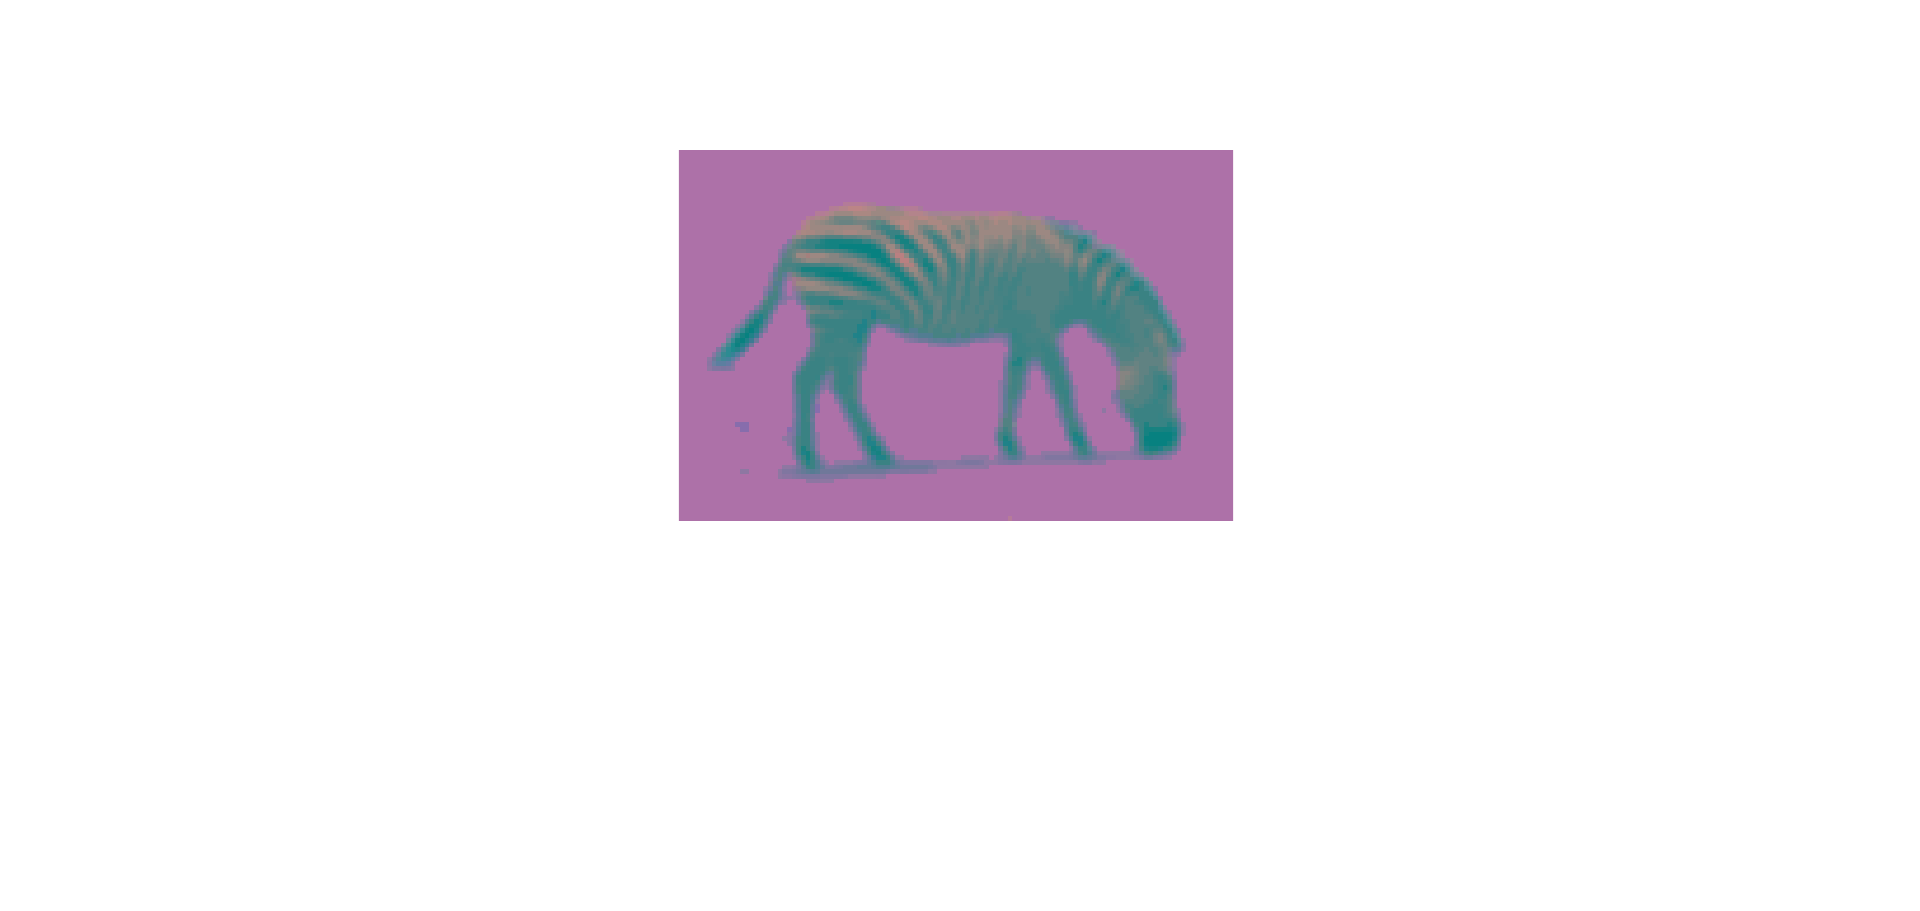
\includegraphics[width=1\linewidth, trim={16cm 9cm 16cm 3cm},clip]{C:/Users/Anton/Desktop/ETH_books/CV/cv_lab05_exercise/last_res/z_2}
			
		\end{minipage}
	\caption{Mean shift algorithm, $r=3$, \texttt{threshold} = 0.01, resized to 0.2 image.}
	\end{center}
\end{figure}
\begin{figure}[h!]
	\begin{center}
		\begin{minipage}[h]{0.49\linewidth}
			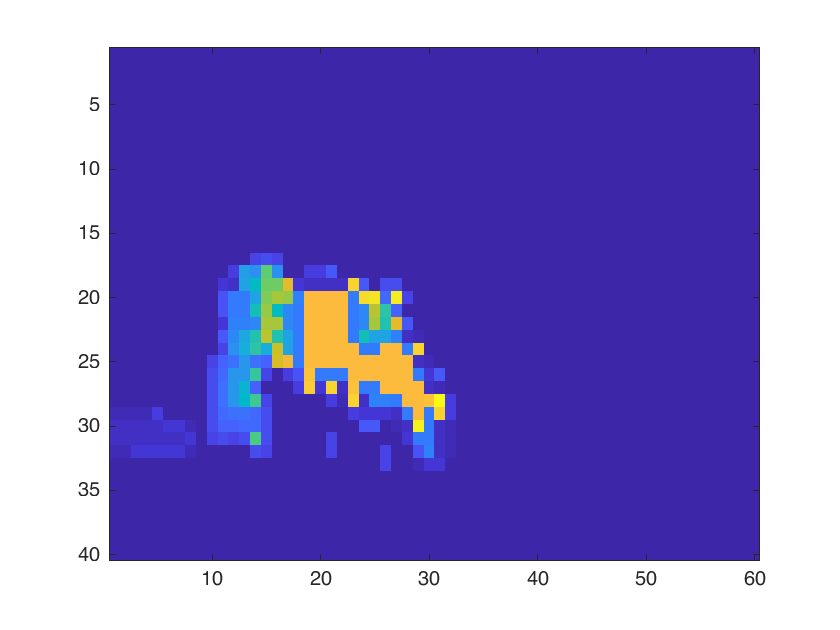
\includegraphics[width=1\linewidth]{C:/Users/Anton/Desktop/ETH_books/CV/cv_lab05_exercise/last_res/cow_02scale_b}			
		\end{minipage}
		\hfill
		\begin{minipage}[h]{0.45\linewidth}
			
\includegraphics[width=1\linewidth, trim={1cm 2cm 1cm 1cm},clip]{C:/Users/Anton/Desktop/ETH_books/CV/cv_lab05_exercise/last_res/cow_02scale_a}	
		\end{minipage}
		\caption{Mean shift algorithm, $r=3$, \texttt{threshold} = 0.01, resized to 0.2 image.}
	\end{center}
\end{figure}
\if 0
\begin{figure}[h!]
	\begin{center}
		\begin{minipage}[h]{0.49\linewidth}
			\includegraphics[width=1\linewidth]{C:/Users/Anton/Desktop/ETH_books/CV/cv_lab05_exercise/results/c_05_3_001a}
		\end{minipage}
		\hfill
		\begin{minipage}[h]{0.49\linewidth}
			\includegraphics[width=1\linewidth, trim={16cm 9cm 16cm 3cm},clip]{C:/Users/Anton/Desktop/ETH_books/CV/cv_lab05_exercise/results/c_05_3_001b}
		\end{minipage}
	\caption{Mean shift algorithm, $r=3$, \texttt{threshold} = 0.01, resized to 0.5 image.}
	\end{center}
\end{figure}
\fi
\textbf{8.3}
We initialize $\mu$ as random points in the range between minimal and maximal values of pixels in the image in every axis. Covariance matrix is initialized as diagonal matrix with values equal to lengths of ranges of pixel values in every corresponding axis.

In further maximization steps we add $10^{-10}I_d$ to the estimated covariance matrices in order to avoid them to become negatively definite because of the rounding (such a small addition practically doesn't change work of the algorithm, but makes it robust).

As a stop condition we use working time (20 min) and iteration (200) constrains + check if log--likelihood $\sum_i \log \sum_k p_i*\mathcal{N}(X_i, \theta_k)$ changed less than for $10^{-4}$ during one step (sums over pixels ($i$) and over clusters ($k$). We use this criterion as it is proved that during EM negative log--likelihood decreases monotonically.

We can compare EM and mean shift algorithms by eye and conclude that the quality of mean shift is better, though it is also much slower. But also its advantage is that it doesn't need prior number of clusters, only parameters which characterize scale of the image but not the color distribution there. Though, is we now how many clusters we should have approximately (we know color composition of the image), then quality of EM could be comparable with than one of mean shift.

Obtained results in res.doc file, first 3 data for zebra images from report.
\begin{figure}[h!]
	\begin{center}
		\begin{minipage}[h]{0.23\linewidth}
			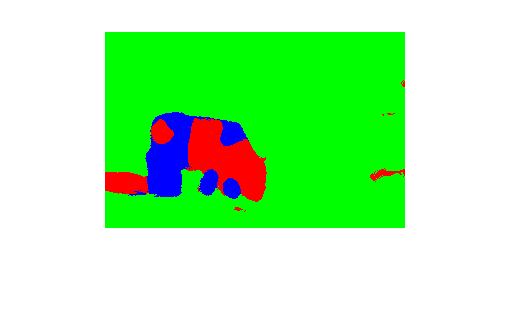
\includegraphics[width=1\linewidth, trim={3cm 2cm 3cm 1cm}, clip]{C:/Users/Anton/Desktop/ETH_books/CV/cv_lab05_exercise/last_res/em_c_3}
		\end{minipage}
		\hfill
		\begin{minipage}[h]{0.23\linewidth}
			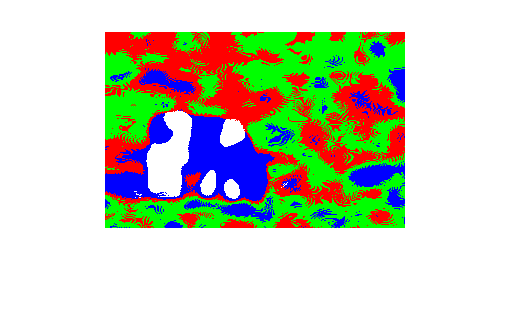
\includegraphics[width=1\linewidth, trim={3cm 2cm 3cm 1cm}, clip]{C:/Users/Anton/Desktop/ETH_books/CV/cv_lab05_exercise/last_res/em_c_4}
		\end{minipage}
	\hfill
	\begin{minipage}[h]{0.23\linewidth}
		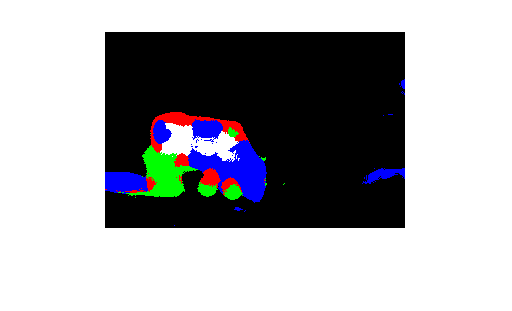
\includegraphics[width=1\linewidth, trim={3cm 2cm 3cm 1cm}, clip]{C:/Users/Anton/Desktop/ETH_books/CV/cv_lab05_exercise/last_res/em_c_5}
	\end{minipage}
\hfill
\begin{minipage}[h]{0.23\linewidth}
	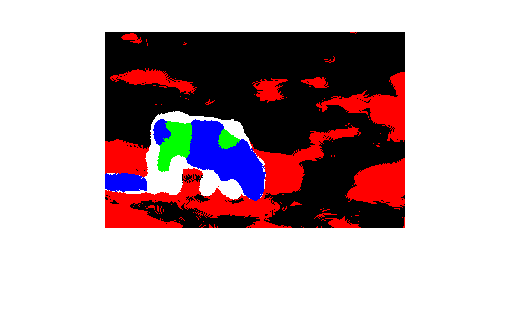
\includegraphics[width=1\linewidth, trim={3cm 2cm 3cm 1cm}, clip]{C:/Users/Anton/Desktop/ETH_books/CV/cv_lab05_exercise/last_res/em_c_5_1}
\end{minipage}
\caption{Result of EM-algorithm for $K=$3, 4, 5 and 5 and full cow image. We can see that for this image $K=3$ is enough and probably the best in terms of the most adequate and simple model, because we have, in general, 3 colors at the picture: black, white and green. Also as it can be seen from all images and especially from comparison of two the most right that the result depends on the initial parameters and becomes more ambiguous with the increase of $K$. Here we can go either in more detailed segmentation of the cow or the grass. So for better result it could be beneficial to start EM several times and find the best for our purposes segmentation somehow. }
	\end{center}
\end{figure}

\begin{figure}[h!]
	\begin{center}
		\begin{minipage}[h]{0.31\linewidth}
			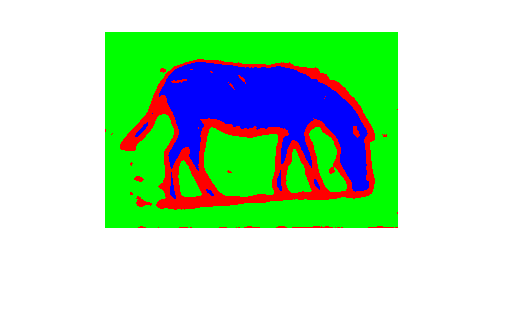
\includegraphics[width=1\linewidth, trim={3cm 2cm 3cm 1cm}, clip]{C:/Users/Anton/Desktop/ETH_books/CV/cv_lab05_exercise/last_res/em_z_3}
		\end{minipage}
		\hfill
		\begin{minipage}[h]{0.31\linewidth}
			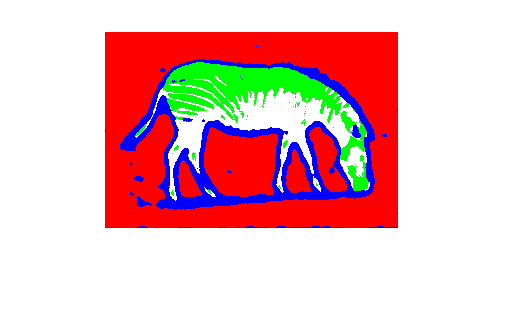
\includegraphics[width=1\linewidth, trim={3cm 2cm 3cm 1cm}, clip]{C:/Users/Anton/Desktop/ETH_books/CV/cv_lab05_exercise/last_res/em_z_4}
		\end{minipage}
		\hfill
		\begin{minipage}[h]{0.31\linewidth}
			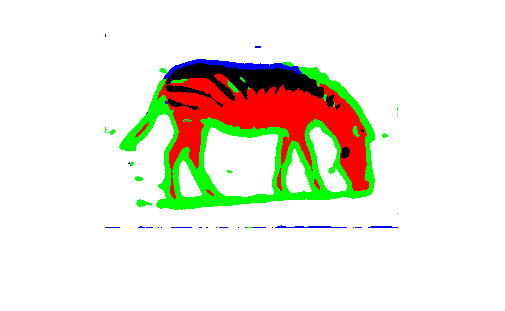
\includegraphics[width=1\linewidth, trim={3cm 2cm 3cm 1cm}, clip]{C:/Users/Anton/Desktop/ETH_books/CV/cv_lab05_exercise/last_res/em_z_5}
		\end{minipage}
		\caption{Result of EM-algorithm for $K=3, 4, 5 and 5$ and zebra image at the 0.5 scale. Because of the more uniform background as it is at the cow image, here different initialization lead to more detailed segmentation of zebra and not grass.}
	\end{center}
\end{figure}
\fi
\begin{center}
	\begin{tabular}{|l|l|l|l|}
		\multicolumn{4}{c}{Resulting parameters of EM for zebra image (pictures in report; analogous data for cow in word file res.doc)}\\
		
	%	\multicolumn{4}{c}{Limit 1000 iterations}\\
		\hline
		$K$ & 3 &  4 &  5 \\
		\hline
		$\alpha_1$&0.18&0.60&0.16\\
		\hline
		$\alpha_2$&0.60&0.12&0.17\\
		\hline
		$\alpha_3$&0.22&0.17&0.025\\
		\hline
		$\alpha_4$&-&0.11&0.59\\
		\hline
		$\alpha_5$&-&-&0.06\\
		\hline
		$\Sigma_1$&
		$10^3 \cdot\bigl( \begin{smallmatrix}1.5452 & -0.1625 & 0.3339\\
		-0.1625 &   0.0476 &  -0.0555\\
		0.3339 & -0.0555  &  0.1162
		\end{smallmatrix}\bigr) $
		&$\bigl( \begin{smallmatrix}64.6580 &   6.9643  & -8.1762\\
		6.9643  & 15.5033 &  -8.6798\\
		-8.1762  & -8.6798  & 11.1971
		
		
		
		\end{smallmatrix}\bigr) $&$\bigl( \begin{smallmatrix}714.3223 &  -3.6447  &  7.3478\\
		-3.6447  &  2.7514 &  -0.2624\\
		7.3478 &  -0.2624 &   6.7077
		
		
	\end{smallmatrix}\bigr) $
		\\
		\hline 	
		$\Sigma_2$&$\bigl( \begin{smallmatrix}65.0278  &  7.0918 &  -8.3061\\
		7.0918  & 15.5652 &  -8.7615\\
		-8.3061 &  -8.7615 &  11.3156
		
		\end{smallmatrix}\bigr) $&$10^3 \cdot\bigl( \begin{smallmatrix}2.2968 &   0.0635  &  0.0184\\
		0.0635 &   0.0107 &   0.0011\\
		0.0184  &  0.0011  &  0.0050
		
		
	\end{smallmatrix}\bigr) $&
	
	$10^3 \cdot\bigl( \begin{smallmatrix}1.4700 &  -0.1963 &   0.3834\\
	-0.1963 &   0.0517 &  -0.0621\\
	0.3834 &  -0.0621  &  0.1263
	
	
	
\end{smallmatrix}\bigr) $\\
		\hline
		$\Sigma_3$&$10^3 \cdot\bigl( \begin{smallmatrix}
		1.6525  &  0.0498 & -0.0044\\
		0.0498  &  0.0085 &  -0.0004\\
		-0.0044 &  -0.0004 &   0.0071
		
		\end{smallmatrix}\bigr) $&
		$10^3 \cdot\bigl( \begin{smallmatrix}    1.3852 &  -0.1413  &  0.2746\\
		-0.1413 &   0.0484 &  -0.0522\\
		0.2746  & -0.0522  &  0.1030
		
		
	\end{smallmatrix}\bigr) $
	&$\bigl( \begin{smallmatrix}86.0880&  -28.6072 &  27.7985\\
	-28.6072 &  71.6477 & -96.4471\\
	27.7985 & -96.4471 & 143.0634
	
	
	
\end{smallmatrix}\bigr) $\\
		\hline
		$\Sigma_4$&-&$\bigl( \begin{smallmatrix}371.8118 &  -9.0585 & -14.4528\\
			-9.0585 &   2.6084 &  -0.8092\\
			-14.4528  & -0.8092  &  9.9131
			
			
			
		\end{smallmatrix}\bigr) $&$\bigl( \begin{smallmatrix}   64.2407 &   7.5333 &  -8.5867\\
		7.5333  & 15.9434 &  -8.7015\\
		-8.5867 &  -8.7015 &  10.8384
		


\end{smallmatrix}\bigr) $\\
		\hline
		$\Sigma_5$&-&-&$\bigl( \begin{smallmatrix}    803.8676 &  -2.2352  &  9.3895\\
			-2.2352 &  11.5380 &  1.9501\\
			9.3895  &  1.9501  &  4.0653
			
			
			
			
		\end{smallmatrix}\bigr) $\\
		\hline
		$\mu_1$&
		$\bigl( \begin{smallmatrix}116.3  &  123.2 &  153.2
	\end{smallmatrix}\bigr)$&
$\bigl( \begin{smallmatrix}170.5  &  114.0 &  168.2
\end{smallmatrix}\bigr)$&
$\bigl( \begin{smallmatrix}67.1  &  130.0 &  130.8
\end{smallmatrix}\bigr)$\\
		\hline
		$\mu_2$&$\bigl( \begin{smallmatrix}170.5  &  114.0 &  168.2
		\end{smallmatrix}\bigr)$&
	$\bigl( \begin{smallmatrix}96.9  &  132.3& 129.6
	\end{smallmatrix}\bigr)$&
$\bigl( \begin{smallmatrix}111.8&123.0&153.5
\end{smallmatrix}\bigr)$\\
		\hline
		$\mu_3$&$\bigl( \begin{smallmatrix}85.1  &  132.0 &  130.5
		\end{smallmatrix}\bigr)$&
	$\bigl( \begin{smallmatrix}120.9  &  122.8 &  154.3
	\end{smallmatrix}\bigr)$&
$\bigl( \begin{smallmatrix} 171.1 & 123.0 & 153.6
\end{smallmatrix}\bigr)$\\
		\hline
		$\mu_4$&-&
		$\bigl( \begin{smallmatrix} 68.0 & 129.7 & 132.0
		\end{smallmatrix}\bigr)$&
	$\bigl( \begin{smallmatrix} 170.5 & 114.0 & 168.2
	\end{smallmatrix}\bigr)$\\
		\hline
		$\mu_5$&-&-&$\bigl( \begin{smallmatrix}130.3 & 134.0 & 129.1
		\end{smallmatrix}\bigr)$\\
		\hline
	\end{tabular}
\end{center}
We can see that the main components with  $\alpha \approx 0.6$ (indexes 2--1--4 in table) and $\alpha =0.17--0.18$ (indexes 1--3--2 in the table) have similar $\mu$ and $\Sigma$ across the different numbers of $K$. So addition of more components just subdivide smaller one to several subclusters, but main two remain.
\if 0
\begin{figure}[h!]
	\begin{center}
		\begin{minipage}[h]{0.6\linewidth}
			\includegraphics[width=1\linewidth]{C:/Users/Anton/Desktop/ETH_books/CV/cv_lab05_exercise/results/pdif}
		\end{minipage}
	\caption{Dependancies of norm of change of probability matrices with different EM-algorithm parameters. Stabilization is achieved (exponential decrease), small peaks show that sometimes configuration of clusters changes leading to more stable one.}
	\end{center}
\end{figure}

\fi
\end{document}